\begin{itemize}
\item
\end{itemize}

\section{Introduction}
Nous répondons dans l'ensemble des documents produits par l'hexanôme H4111 à l'appel d'offre lancé par le COPEVUE visant à concevoir un Système de monitoring à distance de sites isolés. Dans ce document sont détaillés avec plus de précisions les constituants  du projet. Nous insisterons donc sur les points de vue organisationnels liés à la conception de notre solution technique.Après avoir resitué le contexte du problème, il s'agira de définir les objectifs ainsi que les contraintes liés à ce type de projet. Sont détaillées aussi dans ce document, les méthodes de travail,la répartition des rôles au sein du groupe d'ingénierie ainsi que le planning de répartition des tâches et des charges de travail. 

\subsection{Présentation du projet}
Le COPEVUE a lancé un appel d'offre dans le cadre de la réalisation d'un système de monitoring de sites isolés. Il s'agit donc de concevoir en premier lieu une solution technique permettant de répondre aux mieux aux exigences fonctionnelles et non fonctionnelles que le COPEVUE formule. De façon synthétique notre équipe va proposer une solution permettant de surveiller des sites naturels difficiles d'accès (souvent à cause des conditions environnementales) et peu peuplés. Dans ces sites isolés sont souvent regroupés des postes de travail et ces zones doivent pouvoir être surveillées en dépit de la distance qui les sépare du bureau de contrôle.

\subsubsection{Contexte du projet}
Notre cas d'étude se limite pour l'instant à considérer une situation simple : comment pouvoir maintenir de manière rentable des réserves de tel ou tel composé à un niveau correct bien que le site de stockage soit situer dans des zones difficiles d'accès ? L'idéal serait donc de pouvoir suivre a distance l'évolution d'un niveau d'un composé en fonction du temps.Le ravitaillement serait ainsi plus raisonnable car on saurait alors la quantité de composant à acheminer sur place. Trouver une solution fonctionnelle à cette problématique permettrait ainsi d'économiser en frais de maintenance mais aussi et surtout d'éviter certaines catastrophe écologique comme par exemple un manque d'eau dans un réservoir lors d'un feu de forêt ou encore une fuite de carburant d'un réservoir de forêt.

\subsubsection{Objectifs du projet}
Les objectifs principaux de ce projet sont pour ainsi dire assez simple conceptuellement parlant, il s'agit en effet de pouvoir surveiller à distance une installation présente sur un site isolé en installant un réseau de capteurs que l'on va pouvoir relevé et maintenir à distance. Dans un deuxième temps, notre sytème permettra de même d'anticiper les pannes et les desagréments au niveau du site à monitorer en générant des alertes au sein d'un site de supervision pouvant être situé à des miliers de kilomètres des sites à surveiller.

\subsubsection{Découpage en phases du projet}
De manière assez classique, la réalisation du système se fera selon le principe de cycle de vie d'un système (cycle en V).
\begin {center}
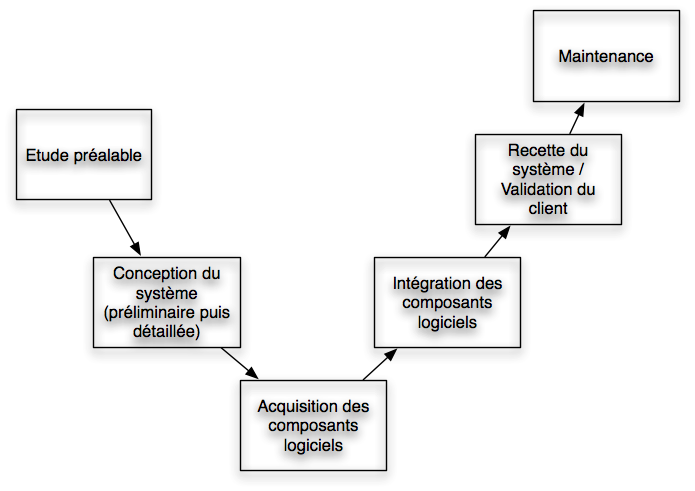
\includegraphics[width=\textwidth]{png/cycleVSysteme.png}
\end {center}

\subsection{Le Plan de Management de Projet}
\subsubsection{Objectifs du PMP}
Ce document a pour objectif de décrire le pilotage de  tout le projet du point de vue du management, c'est à dire l'approche organisationnelle, l'approche produit, l'approche temporelle/charge de travail, les aspects financiers. Il est important de voir que ce dossier ne constitue qu'un draft et qu'ainsi, certaines parties seront volontairement non exhaustives voir incomplètes.

\section{Organisation du projet et différents acteurs}
\subsection{La maitrise d'ouvrage}
La maitrise d'ouvrage sera représentée par la comission européenne COPEVUE en charge de l'envoi de l'appel d'offre aux différents bureaux d'études. Il pourra être intéressant de mettre en oeuvre un site dit tampon ou de référence permettant de tester en temps réel les améliorations apportées au système. Ce système pourra être testé en présence de représentants du
 COPEVUE pour attester de l'avancée du travail.
\subsection{La maitrise d'oeuvre}
L'équipe de travail en charge de ce projet sera augmentée de quelques personnes par rapport à l'équipe en charge de la réponse à l'appel d'offre.
Notre groupe se compose donc au final de :

\begin{itemize}
\item Le Chef de projet.
\item Le Responsable qualité.
\item Le Responsable du déploiement du système.
\item Le Responsable du pôle R\&D.
\item Une équipe commerciale.
\end{itemize}
Le pôle R\&D étant constitué d'ingénieur chargé de maintenir le système mais aussi de le faire évoluer.
Le Responsable du déploiement est quant à lui chargé de manager les techniciens qui intègrent le système mais aussi de reporter les éventuels bugs d'intégration à l'équipe R\&D.

\subsection{Documents de références}
\begin{itemize}
\item Aide à la rédaction d'une procédure
\item Dossier d'initialisation
\item Procédure de décomposition d'un système en sous-systèmes et sous projets
\end{itemize}

\section{Démarche de développement du système}
D'après le cycle de vie du système décrit plus haut, il est nécessaire de se rendre compte qu'il faut découper le système en briques élémentaire avant tout début de travail de réalisation. Le système complexe doit donc être réparti en différents sous système qui eux mêmes donneront lieu à la rédaction de plusieurs cahiers des charges. Les cahiers des charges ne doivent pas se limiter aux parties logicielles mais doivent prendre en compte de même les projet matériels, d'intégration, de formation de l'équipe de maîtrise d'oeuvre.

\subsection{Rappel de la méthode de découpage d'un système en sous système}

\begin {center}
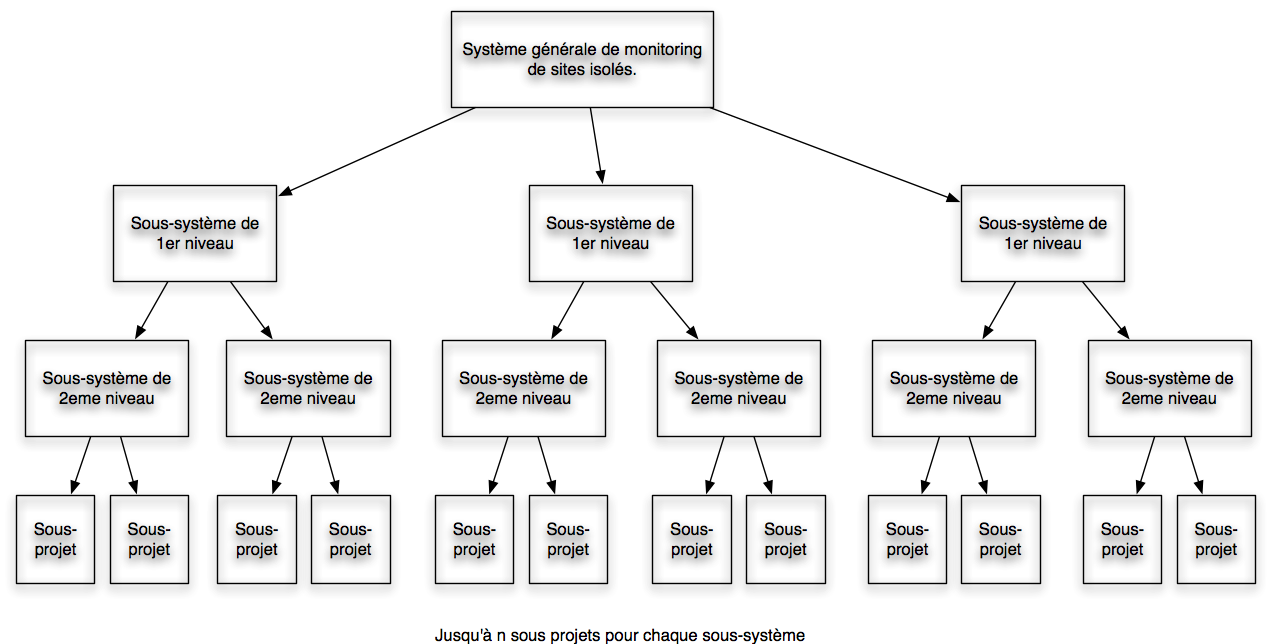
\includegraphics[width=\textwidth]{png/decoupageType.png}
\end {center}

Le premier niveau de découpage d'un système en sous systèmes dissocie les différents domaines fonctionnels présent au sein du système à construire. Dans un deuxième temps, il s'agit de s'intéresser plus aux découpages logiciels/matériels qui peuvent être fait pour chaque sous-système représentant un domaine fonctionnel.
Ensuite, chaque sous-système de 2ème niveau va donner lieu à l'établissement de cahiers des charges. Ces cahiers des charges seront les résultats (en termes de livrables) de la décomposition des sous-systèmes en sous projets. Lorsque l'on rédige les cahiers des charges touchant aux différents sous projets, l'équipe se fait une idée très précise de comment doit s'articuler le système.

\subsection{Découpage du système monitoring de sites isolés}
Nous avons découpé notre système en suivant le document de référence \og Décomposition d'un système en sous-systèmes et sous-projet".

\subsubsection{Découpage du système en sous-systèmes}

%TODO Mettre en landcape ce png.
\begin {center}
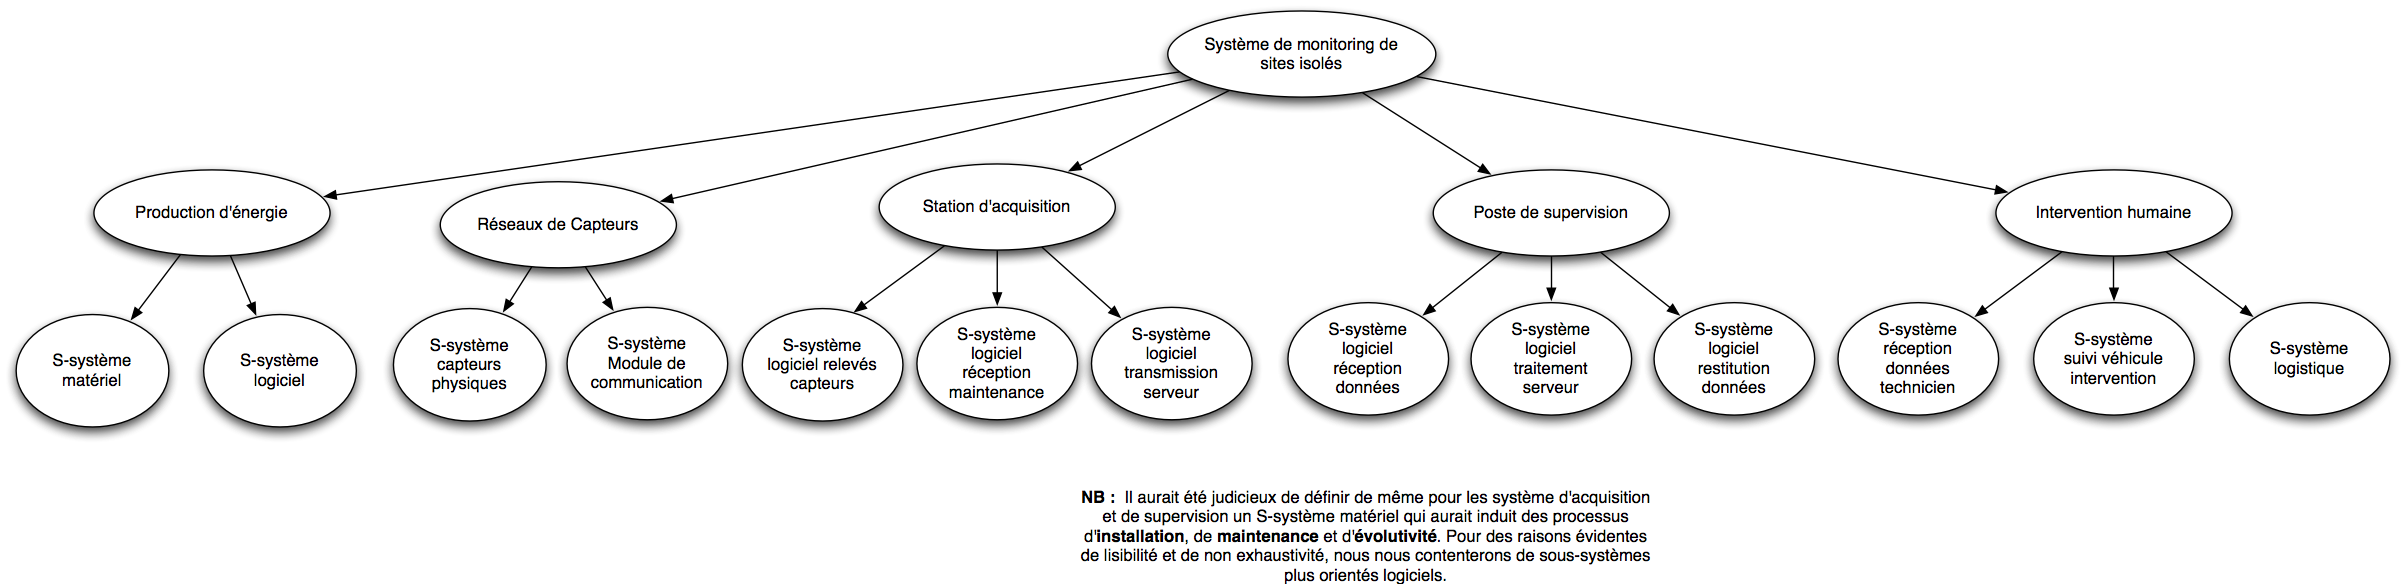
\includegraphics[width=\textwidth]{png/graphDecompoSousSystemes.png}
\end {center}

\subsubsection{Identification des projets et sous-projets}
Pour chaque système, voici leurs décompositions en sous projets. Nous insistons beaucoup sur les projets logiciels et certains projets plus \og généraux \fg ne figurent donc pas sur ce documents.

\begin {center}
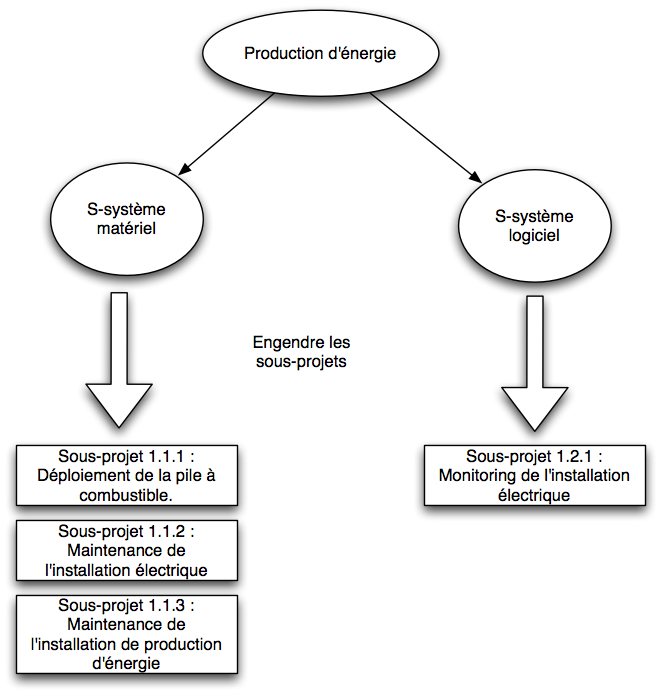
\includegraphics[width=\textwidth]{png/ss1ProdE.png}
\caption{Découpage en sous-projets du sous-système production d'énergie}
\end {center} 

\begin {center}
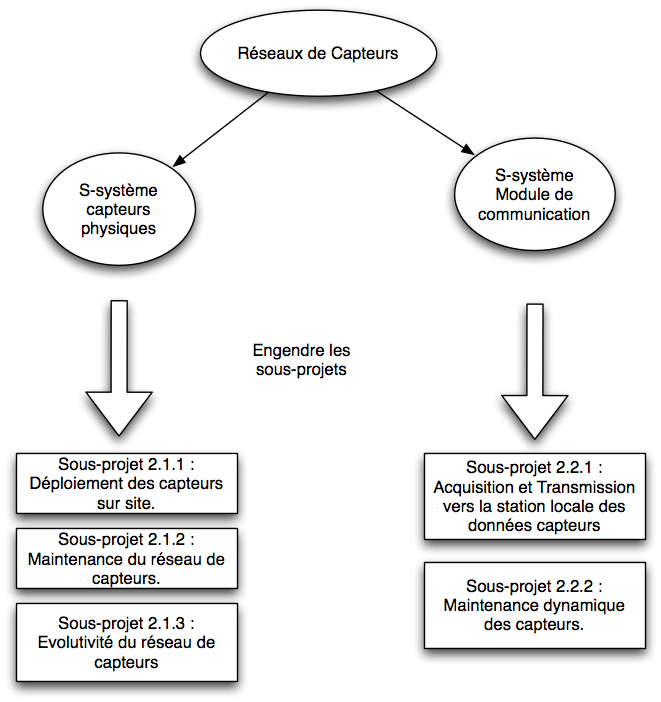
\includegraphics[width=\textwidth]{png/ss1Capteurs.png}
\caption{Découpage en sous-projets du sous-système capteurs}
\end {center}

\begin {center}
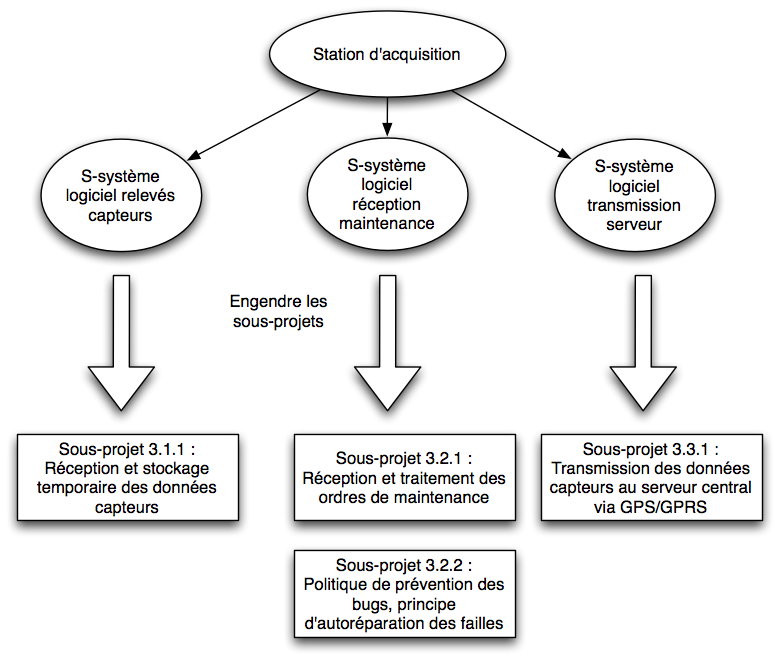
\includegraphics[width=\textwidth]{png/ss3Station.png}
\caption{Découpage en sous-projets du sous-système station d'acquisition}
\end {center}

\begin {center}
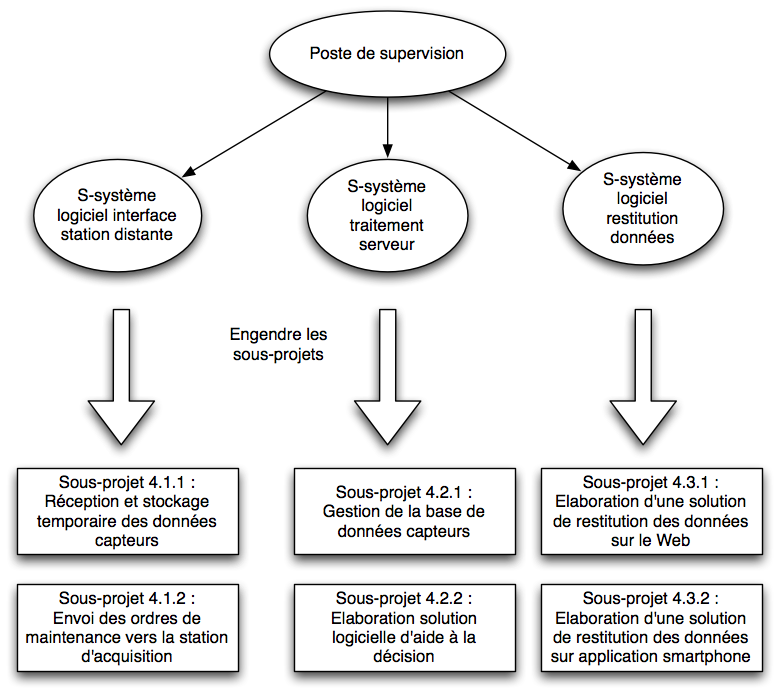
\includegraphics[width=\textwidth]{png/ss4Supervision.png}
\caption{Découpage en sous-projets du sous-système supervision}
\end {center}
\begin {center}

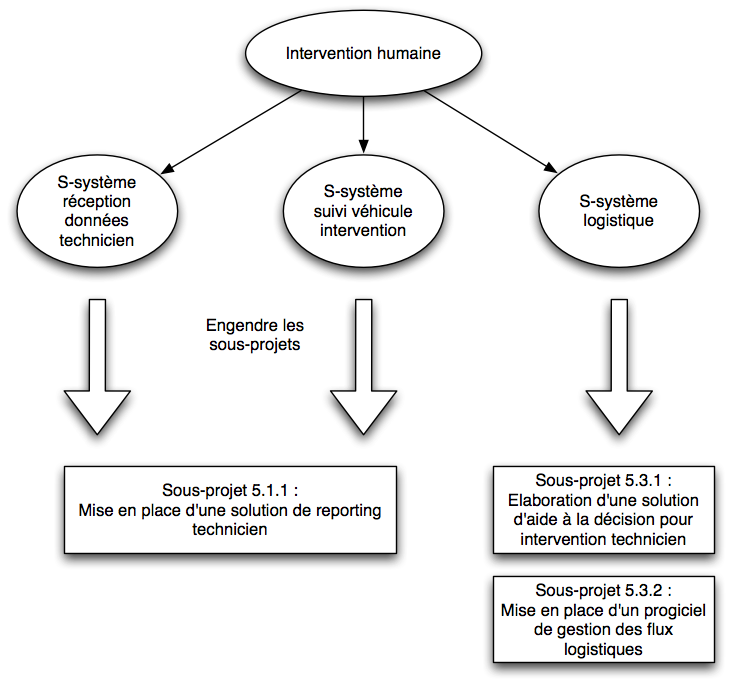
\includegraphics[width=\textwidth]{png/ss5IH.png}
\caption{Découpage en sous-projets du sous-système intervention humaine}
\end {center}


\subsection{Description des sous-projet}

\begin{itemize}
\item Sous-projet 1.1.1 : Le déploiement de la pile à combustible consiste dans un premier temps en l'acquisition du matériel à installer sur place au niveau du site isolé à savoir le reservoir d'hydrogène ainsi que le générateur qui transforme de cette hydrogène préssurisé en éléctricité. Il est donc nécessaire de disposer du matériel nécessaire pour réaliser cette installation à savoir :  2 ou 3 techniciens selon la taille du site à monitorer, un camion équipé en outils mais aussi équipé d'un lieu à vivre pour pouvoir éventuellement loger les techniciens le temps de l'installation du système de production d'énergie. Le camion doit pouvoir être traçable par GPS et les techniciens doivent éffectué leur reporting quotidiennement.
\item Sous-projet 1.1.2 : La maintenance de l'installation électrique doit pouvoir être faite à distance. Pour cela il est nécessaire d'avoir un bilan de l'état de marche de la station. Il est donc nécessaire que des capteurs soient installés au niveau des installations électriques pour guetter un éventuel problème de fonctionnement du système. Ce système de maintenance/supervision permet donc d'anticiper les pannes et le cas échéant, de faire intervenir un techicien sur zone. L'installation des outils de relevé de la santé du système électrique devront être fait en même temps que la mise en marche de la station d'acquisition des données capteurs car c'est elle qui va relayer l'information vers le poste de supervision.
\item Sous-projet 1.1.3 : La maintenance de l'installation de production d'énergie devra être planifiée, il sera donc nécessaire d'envoyer des techniciens de manière très espacé dans le temps (tout les ans ou tout les deux ans) afin de vérifier l'état de la pile à hydrogène. Cette vérification est obligatoire et ne remet pas en cause le sous-projet précédent permettant de dresser le bilan de santé en temps réel de l'installation électrique. Ce type de travail peut être réalisé par un technicien seul. Le principe étant qu'un technicien puisse réviser toute les stations d'une zone en se déplaçant avec son camion. De même, ce technicien est tenu au reporting quotidien via l'interface smartphone de la plateforme de supervision.
\item Sous-projet 1.2.1 : Le monitoring de l'installation électrique consistera en la restitution des informations renvoyées par les capteurs vers le centre de supervision. Lors d'un problème technique nécessitant de se déplacer, une fiche d'intervention sera formulée et adressée au technicien en charge du site. Cette fiche décrira le problème, rappelera les éventuelles étapes de réparation et prodiguera des conseils pratiques aidant le technicien. Tout ceci sera donc accessible au technicien par le biais de son interface smartphone.
\medskip
\item Sous-projet 2.1.1 : Le déploiement des capteurs sur site sera éffectué de la même façon que pour le déploiement de la pile a hydrogène. Après l'acquisition matérielle des capteurs et la préparation de ceux-ci pour l'installation sur site, un groupe de technicien sera chargé d'installer physiquement ces capteurs sur site suivant les plans fournis par la R\&D. En plus des techniciens, il peut être intéressant qu'un ingénieur puisse manager le projet au sein du site isolé afin de palier aux éventuels problèmes de dernière minute.
\item Sous-projet 2.1.2 : La maintenance du réseau de capteurs sera en lien étroit avec la maintenance de l'installation électrique. Il s'agit donc d'anticiper les causes de pannes possibles et de les signaler au superviseur. De la même façon que précedemment, lors d'un grave problème technique, on enverra un technicien sur place. Le but final étant de limiter au maximum l'intervention humaine sur site car celle-ci est longue et très couteuse.
\item Sous-projet 2.1.3 : L'évolutivité du réseau de capteurs sera discutée entre le COPEVUE et l'équipe de R\&D présente au sein de notre entreprise. Il doit être rapidement possible de déployer un nouveau type de capteurs sur site afin de répondre à un nouveau besoin. Ce sous-projet peut-être lancé à n'importe quel moment de la phase de vie de notre système.
\item Sous-projet 2.2.1 : L'acquisition et la transmission vers la station locale des données capteurs. Il s'agit donc de développer un logiciel capable de faire l'interface entre les capteurs déployés sur le site isolé et la station locale représentée par une carte d'acquisition. La transmission qui se fera sans fil à intervales réguliers impliquera que la station locale soit en état "réveillée" pour pouvoir réceptionner les informations. Le logiciel sera développé et testé en interne avant son déploiement. L'équipe de développement attachera une grande importance à la stabilité et à la robustesse du système.
\item Sous-projet 2.2.2 : La maintenance dynamique est l'interface logicielle du projet de maintenance du réseau de capteurs.
\medskip
\item Sous-projet 3.1.1 : La réception et le stockage temporaire des données capteurs permet de spécifier comment les données capteurs vont être gardées au sein de la carte d'acquisition. Le but étant de les garder le temps le plus court possible et de les transmettre assez rapidement afin d'économiser de l'énergie sur le site.
\item Sous-projet 3.2.1 : La réception est le traitement des ordres de maintenance. La station sera à l'écoute d'ordre de maintenance arrivant du poste de supervision permettant par exemple de réinitialiser le système lors de l'apparition d'un problème grave. Il faut donc spécifier l'interface entre ces deux systèmes et définir un jeu de commandes que l'on va pouvoir exécuter à distance.
\item Sous-projet 3.2.2 : Mise en place lors des phases de développement d'un système d'\og autoréparation du système d'acquisition, notre groupe n'a pas vraiment creusé ce point mais ressent le besoin d'un tel dispositif permettant au système isolé d'apprendre de ses erreurs à la manière par exemple des robots de la nasa envoyés sur une autre planète (d'une façon plus modeste bien entendu).
\item Sous-projet 3.3.1 : Module de transmission des données capteurs vers le centre de supervision. Il est nécessaire de pouvoir switcher rapidement entre la technologie GPS et GPRS et de pouvoir assurer l'intégrité des donnés. Les requète d'envoi des données seront faites via le protocole HTTP.
\meskip 
\item Sous-projet 4.1.1 : Réception et stockage des données capteurs par le site de supervision central. Ces données seront stockées dans des bases de données et accessible via des requètes SQL. Il est important de dater les données afin de pouvoir exploiter et tracer l'évolution des données en fonction du temps.
\item Sous-projet 4.1.2 : Envoi des ordres de maintenance vers la station d'acquisition par le centre de supervision. Ces ordres pourront être envoyés de manière automatique ou être initiés par les agents de supervision. Cette envoi d'ordre de maintenance implique de définir un protocole de communication entre le poste de supervision et la station d'acquisition sur site.
\item Sous-projet 4.2.1 et 4.2.2 : Gestion de la base de données capteurs et Elaboration d'une solution logicielle d'aide à la décision. Il s'agit ici de pouvoir déleguer une partie de l'analyse des données capteurs à la machine qui gère la base de données. Ce logiciel permettra par exemple de générer des alertes en fonction des niveau seuil de chaque capteurs. Il sera possible d'enrichir à tout moment le système à la manière d'un système expert.
\item Sous-projet 4.3.1 : Elaboration d'une solution de restitution des données sur le web. Ce sous-projet concerne la création d'une interface web permettant de mettre en forme les données capteurs ainsi que les alertes générées par le système d'aide à la décision. Dans ce sous-projet logiciel on accordera une attention particulière à la clarté et à l'ergonomie de l'IHM. Ce sous-projet inclus de même le processus d'envoi des ordes de maintenance vers la station d'acquisition. Il s'agit de l'interface entre le superviseur et le site isolé.
\item Sous-projet 4.3.2 : L'élaboration d'une solution de restitution des données sur application smartphone permettra au technicien de disposer d'informations très précise sur l'état du site isolé. Les informations seront communes à l'interface web puisqu'issues de la même base de données.
\item Sous-projet 5.1.1 : La mise en place d'une solution de reporting technicien sera implémenté sous différentes plateformes à savoir l'interface web et l'application smartphone. L'application smartphone devra permettre le reporting du technicien au moment de son intervention. Ce reporting sera transmis puis mis à disposition du superviseur via l'interface web.
\item Sous-projet 5.3.1 : Mise en place d'une solution d'aide à la décision pour l'intervention du technicien. Via l'interface web ou l'application smartphone, le technicien sera conseillé sur la manière de regler tel ou tel problème lorsqu'il est sur site. Les plans ainsi que les manuels des capteurs numérisés seront interprétés et les informations importantes pourront être restituées au techniciens.
\item Sous-projet 5.3.2 : Intégration d'un progiciel de gestion des flux logistiques. Afin de positionner le camion d'intervention, savoir quand l'envoyer sur site, faire l'inventaire des outils nécessaires à une intervention.
%TODO Continuer.
\end{itemize}


\subsubsection{Choix des projets retenus pour établissement cahier des charges}
Chaque projet défini plus haut va amener à l'établissement d'un cahier des charges. En ce qui concerne notre groupe de travail, nous avons décidé de rédiger :

\begin{itemize}
\item Cahier des charges du sous-projet 2.2.1 : Acquisition et transmission vers la station locale des données capteurs.
\item Cahier des charges du sous-projet 3.3.1 : Transmission des données capteurs au serveur central via GPS/GPRS.
\item Cahier des charges du sous-projet 4.3.1 : Elaboration d'une solution de restitution des données sur le Web.
\end{itemize}

\section{Moyens à mettre en oeuvre}

\subsection{Moyens matériels}
\subsection{Moyens logiciels}
Listes des différents outils et méthodes qui seront utilisés tout au long du projet:
\begin{itemize}
\item \textbf{Google Docs} : Outil en ligne permettant un partage et un travail simultané en temps réel sur différents types de documents, avec une gestion des versions. Ne sera utilisé que le temps de la mise en place d’outils plus avancés.
\item \textbf{UML} : langage de modélisation, qui sera surtout utilisé pour la modélisation des cas d’utilisation.
\item \textbf{Redmine} : Gestionnaire de projet en ligne, disposant d’un wiki, permettant de suivre le temps passé sur une tâche, d’attribuer les tâches aux différents utilisateurs, de créer un  diagramme de Gantt pour faciliter le travail du chef de projet.
\item \textbf{Git} : Gestionnaire de sources, qui sera intégré directement à Redmine, permettant de travailler à plusieurs sur un même document et de résoudre facilement les conflits au moment de la mise en commun.
\item \textbf{LaTeX} : Langage et système de composition de documents, qui a l’avantage d’être textuel, et donc plus facile à versionner que des documents binaires Office.
\item \textbf{Diagramme de Gantt } : Outil permettant l’ordonnancement et la visualisation des tâches entre les différents membres du projet, afin de gérer au mieux l’avancement du projet.
\end{itemize}
Pour faire le développement des produits logiciels, il pourra être intéressant d'utiliser le framework .NET permettant de rendre des applications facilement portables sur internet. Ceci est important vis à vis de notre choix de vouloir rendre les informations disponibles via un site web.

\subsection{Moyens humains}
Comme définit au dessus, nous avons.
\begin{itemize}
\item Le Chef de projet.
\item Le Responsable qualité.
\item Le Responsable du déploiement du système.
\item Le Responsable du pôle R\&D qui sera à la tête d'une équipe de 10 personnes en charges du développement des logiciel et du déploiement des infrastructures matérielles informatiques.
\item Une équipe commerciale.
\item Une équipe de technicien qui sera en charge d'intervenir sur les sites à problèmes.
\end{itemize}
Le pôle R\&D étant constitué d'ingénieur chargé de maintenir le système mais aussi de le faire évoluer.
Le Responsable du déploiement est quant à lui chargé de manager les techniciens qui intègrent le système mais aussi de reporter les éventuels bugs d'intégration à l'équipe R\&D.
\subsubsection{Evaluation des charges de travail}
non défini dans ce draft.






